\documentclass[10pt,a4paper]{article}
\usepackage[margin=2cm]{geometry}
\usepackage{amsmath,amssymb}
\usepackage{graphicx,booktabs,xcolor}
\usepackage{listings}
\usepackage[colorlinks=true,linkcolor=blue!50!black,urlcolor=blue!50!black]{hyperref}
\usepackage{microtype}

\lstset{language=Python,basicstyle=\ttfamily\small,keywordstyle=\color{blue!60!black}\bfseries,
  commentstyle=\color{green!40!black},stringstyle=\color{red!50!black},
  frame=single,framerule=0.3pt,rulecolor=\color{gray!60},backgroundcolor=\color{gray!5},
  columns=fullflexible,keepspaces=true,showstringspaces=false,
  numbers=left,numberstyle=\tiny\color{gray},xleftmargin=1.5em,aboveskip=6pt,belowskip=4pt}
\newcommand{\code}[1]{\texttt{#1}}
\newcommand{\dev}{\operatorname{dev}}
\newcommand{\Th}{\mathcal{T}_h}
\newcommand{\Fh}{\mathcal{F}_h}
\setlength{\parindent}{0pt}\setlength{\parskip}{4pt}\setlength{\emergencystretch}{3em}\sloppy

\title{\vspace{-1.2cm}Mass Conserving Mixed Stress (MCS) Methods in NGSolve\\[2pt]
\large Spaces, formulation and NGSolve syntax}
\author{Philip Lederer, Xaver Mooslechner, Jay Gopalakrishnan,\\ Christopher Lackner, Joachim Sch\"oberl}
\date{NGSolve Technical Note 2026-03\quad$\bullet$\quad November 2026}

\begin{document}
\maketitle\vspace{-0.9cm}

\section{The method}

We consider the Stokes problem with viscosity $\nu$:
\[
  -\operatorname{div}\bigl(2\nu\,\varepsilon(u)\bigr) + \nabla p = f, \qquad \operatorname{div} u = 0 \quad\text{in } \Omega,
\]
with Dirichlet data $u = g$ on $\Gamma_D$ and the do-nothing condition $(2\nu\varepsilon(u) - pI)\,n = 0$ on $\Gamma_N$.
The MCS method \cite{gls1,lederer} introduces the deviatoric viscous stress $\sigma = 2\nu \dev\varepsilon(u)$ as an additional unknown. Its main properties are:
\begin{itemize}\setlength\itemsep{1pt}
\item The velocity is $H(\operatorname{div})$-conforming and the pressure space is exactly $\operatorname{div} V_h$, so $\operatorname{div} u_h = 0$ \emph{pointwise}. The method is pressure robust: velocity errors do not depend on $p/\nu$.
\item The stress is \emph{normal-tangential} continuous ($\sigma \in H(\operatorname{curl}\operatorname{div})$). Through $\sigma_{nt}$, it enforces the missing tangential continuity of $u_h$ weakly.
\item Hybridization by a facet variable $\hat u$ (the tangential velocity) makes all stress and higher-order velocity/pressure dofs element-local. After static condensation only facet unknowns remain.
\item Symmetry of $\sigma$ is imposed weakly by a skew-symmetric Lagrange multiplier $\eta$ (\emph{MCS with weak symmetry} \cite{gls2}). Without it, one uses the simpler gradient form $\sigma = \nu\dev\nabla u$.
\end{itemize}

\paragraph{Discrete formulation (hybrid, weakly symmetric).}
Find $(u_h,\sigma_h,\hat u_h,p_h,\eta_h) \in V_h\times\Sigma_h^{dc}\times\hat V_h\times Q_h\times W_h$ such that for all test functions
\begin{align*}
  \tfrac{1}{2\nu}(\sigma_h,\tau) - b(\tau,(u_h,\hat u_h)) + (\tau,\eta_h) &= 0 && \forall\, \tau \in \Sigma_h^{dc},\\
  -b(\sigma_h,(v,\hat v)) + (\operatorname{div} v, p_h) &= -(f,v) && \forall\, (v,\hat v) \in V_h\times\hat V_h,\\
  (\operatorname{div} u_h, q) = 0, \qquad (\sigma_h,\xi) &= 0 && \forall\, q\in Q_h,\ \xi\in W_h,
\end{align*}
with the distributional divergence pairing, written element by element:
\[
  b(\tau,(v,\hat v)) \;=\; \sum_{T\in\Th}\Bigl( \int_T \tau : \nabla v \,dx \;-\; \int_{\partial T} (\tau n)_t\cdot(v_t - \hat v_t)\,ds \Bigr),
  \qquad w_t := w - (w\cdot n)\,n .
\]
The first equation states $\sigma_h = 2\nu(\dev\nabla u_h - \eta_h)$. Together with $(\sigma_h,\xi)=0$ this gives $\eta_h \approx \operatorname{skw}\nabla u_h$, hence $\sigma_h \approx 2\nu\dev\varepsilon(u_h)$.
For the \textbf{gradient form}, drop $\eta,\xi$ and replace $\tfrac{1}{2\nu}$ by $\tfrac1\nu$.
The velocity Dirichlet condition is split: $u\cdot n = g\cdot n$ on $V_h$ and $\hat u = g_t$ on $\hat V_h$. The do-nothing condition is natural.

\section{The spaces}

Let $k\ge 1$ be the velocity order, $\Th$ the mesh and $\Fh$ its facets. All spaces below are created from the velocity space alone. The order rules have been checked to be stable (injectivity of the discrete divergence, optimal convergence) on trigs, quads, tets, prisms and hexes.

\begin{description}\setlength\itemsep{3pt}
\item[Velocity] \code{V = HDiv(mesh, order=k)}.
  On simplices the default is BDM: $V_h = \{v\in H(\operatorname{div}): v|_T \in P_k(T)^d\}$. On quads, prisms and hexes the default is the tensor-product Raviart--Thomas element. For prisms this is $RT_k(\text{trig})\otimes P_k \,\oplus\, P_k(\text{trig})\otimes P_{k+1}\,e_z$. The flag \code{RT=True/False} (or \code{trigRT}, \code{tetRT}, \dots\ per element type) overrides the default; see Technical Note 2026-01.

\item[Pressure] \code{Q = V.CreateDivergenceSpace()} gives $Q_h = \operatorname{div} V_h$ exactly, element by element:
  $P_{k-1}(T)$ for BDM, and for RT $P_k(T)$ on simplices, $Q_k$ on quads/hexes, $P_k\otimes P_k$ on prisms.
  Element constants are global (wirebasket) dofs. All higher modes are local, so they are removed by static condensation.

\item[Stress] \code{S = V.CreateStressSpace()} returns \code{HCurlDiv(mesh, order=k-1, orderinner=k)}:
  \[
    \Sigma_h=\Bigl\{\tau\in L^2(\Omega)^{d\times d}:\ \begin{aligned}[t]&\operatorname{tr}\tau=0,\ \ \tau|_T \text{ polynomial of degree }k,\\
      &\tau_{nt}:=(\tau n)_t \text{ continuous across } \Fh,\ \ \tau_{nt}|_F\in P_{k-1}(F)^{d-1}\Bigr\},\end{aligned}
  \]
  with $Q_{k-1}(F)$ on quadrilateral facets. On simplices, $\Sigma_h = \{\tau\in\dev P_k:\ \tau_{nt}|_F\in P_{k-1}\}$ is the original MCS stress space.
  The same space serves the gradient form and the weakly symmetric form. A computed inf-sup constant of the full system shows no need for the Gopalakrishnan--Guzm\'an bubbles \cite{gg} there, on trigs and tets alike.
  The only special case is RT velocities of order $1$ on trigs. There \code{orderinner=1} plus \code{GGbubbles} is used: 8 local dofs instead of 12 for \code{orderinner=2}, with the same quadrature order.
  To inspect what was chosen, use \code{print(S.flags)}.
  An explicit \code{order=...} switches the automatic choice off. Other keyword arguments are passed to \code{HCurlDiv}.

\item[Hybridized stress] \code{Sdc = Discontinuous(S)} breaks the $\tau_{nt}$-continuity, so $\Sigma_h^{dc} = \prod_T \Sigma_h|_T$ consists of local dofs only.
  \code{Sdc.base\_space} gives back the conforming space \code{S}.

\item[Tangential velocity] \code{Vhat = Sdc.CreateMultiplierSpace()} is \code{TangentialFacetFESpace(mesh, order=k-1)}:
  \[
    \hat V_h = \{\hat v \in L^2(\Fh)^d:\ \hat v\cdot n = 0,\ \ \hat v|_F \in P_{k-1}(F)^{d-1}\}.
  \]
  Its degree matches $\tau_{nt}$ exactly. Therefore $\{\tau \in \Sigma_h^{dc}: \sum_T\int_{\partial T}\tau_{nt}\cdot\hat v = 0\ \forall \hat v\} = \Sigma_h$, and the hybrid and the conforming method give identical solutions.

\item[Symmetry multiplier] \code{W = Sdc.base\_space.CreateSymmetryMultiplierSpace()} is \code{MatrixValued(L2(mesh, order=k-1), skewsymmetric=True)}:
  \[
    W_h = \{\eta \in L^2(\Omega)^{d\times d}:\ \eta = -\eta^T,\ \eta|_T\in P_{k-1}(T)\}.
  \]
  Its proxy is a skew-symmetric matrix, so the constraint is just \code{InnerProduct(sigma, xi)*dx}.
\end{description}

\begin{table}[h]\centering\small
\begin{tabular}{@{}llll@{}}\toprule
 element & velocity default & $Q_h$ & $\Sigma_h$ (facet, inner)\\\midrule
 trig  & BDM$_k$ & $P_{k-1}$ & $(k-1,\,k)$; RT$_1$: $(0,1)$ + GG bubbles\\
 quad  & RT$_k$ (tensor) & $Q_k$ & $(k-1,\,k)$\\
 tet   & BDM$_k$ & $P_{k-1}$ & $(k-1,\,k)$\\
 prism & RT$_k$ (tensor) & $P_k\otimes P_k$ & $(k-1,\,k)$\\
 hex   & RT$_k$ (tensor) & $Q_k$ & $(k-1,\,k)$\\\bottomrule
\end{tabular}
\caption{What the creator functions return. Mixed meshes (e.g.\ tet + prism boundary layers) use the same rules element by element.}
\end{table}

\section{A complete example}

Stokes flow around a cylinder in the DFG channel. The velocity order is $k=3$, with weak symmetry and hybridization. \code{Solve} detects the local dofs and applies static condensation automatically.

\begin{lstlisting}
from ngsolve import *
from netgen.occ import Rectangle, Circle, X, Y

rect = Rectangle(2.2, 0.41).Face()
rect.edges.Min(X).name = "inlet"
rect.edges.Max(X).name = "outlet"
rect.edges.Min(Y).name = rect.edges.Max(Y).name = "wall"
cyl = Circle((0.2, 0.2), 0.05).Face()
cyl.edges.name = "cyl"
mesh = (rect - cyl).GenerateMesh(dim=2, maxh=0.05)
mesh.Curve(3)

k, nu = 3, 1e-3
V    = HDiv(mesh, order=k)                                 # velocity
S    = Discontinuous(V.CreateStressSpace())                # stress, hybridized
Vhat = S.CreateMultiplierSpace()                           # tangential velocity
Q    = V.CreateDivergenceSpace()                           # pressure = div V
W    = S.base_space.CreateSymmetryMultiplierSpace()        # skew-symmetric multiplier

(u, sigma, uhat, p, eta), (v, tau, vhat, q, xi) = (V*S*Vhat*Q*W).TnT()

n = specialcf.normal(2)
tang = lambda w: w - (w*n)*n
def B(tau, v, vhat):
    return InnerProduct(tau, Grad(v))*dx - tang(tau*n)*tang(v-vhat)*dx(element_boundary=True)

a = (1/(2*nu)*InnerProduct(sigma, tau)*dx - B(tau, u, uhat) - B(sigma, v, vhat)
     + div(u)*q*dx + div(v)*p*dx
     + InnerProduct(sigma, xi)*dx + InnerProduct(tau, eta)*dx)

uin = CF((1.5*4*y*(0.41-y)/0.41**2, 0))
gf = Solve(a == 0, u[BND("inlet")] == uin, uhat[BND("inlet")] == uin,
           u[BND("wall|cyl")] == 0, uhat[BND("wall|cyl")] == 0)
uh, sh, ph = gf[u], gf[sigma], gf[p]
\end{lstlisting}

For a body force, write \code{a == -f*v*dx}. Without weak symmetry, drop \code{W}, \code{eta}, \code{xi} and use \code{1/nu} in the first term.
The space \code{V*S*Vhat*Q*W} has 47\,840 dofs; after condensation only the facet dofs of \code{V} and \code{Vhat} and the element constants of \code{Q} remain.
The run takes about one second on a laptop. The computed velocity satisfies $\|\operatorname{div}u_h\|_{L^2} = 6\cdot10^{-15}$.

\begin{figure}[h]\centering
\begin{minipage}[c]{0.64\textwidth}\centering
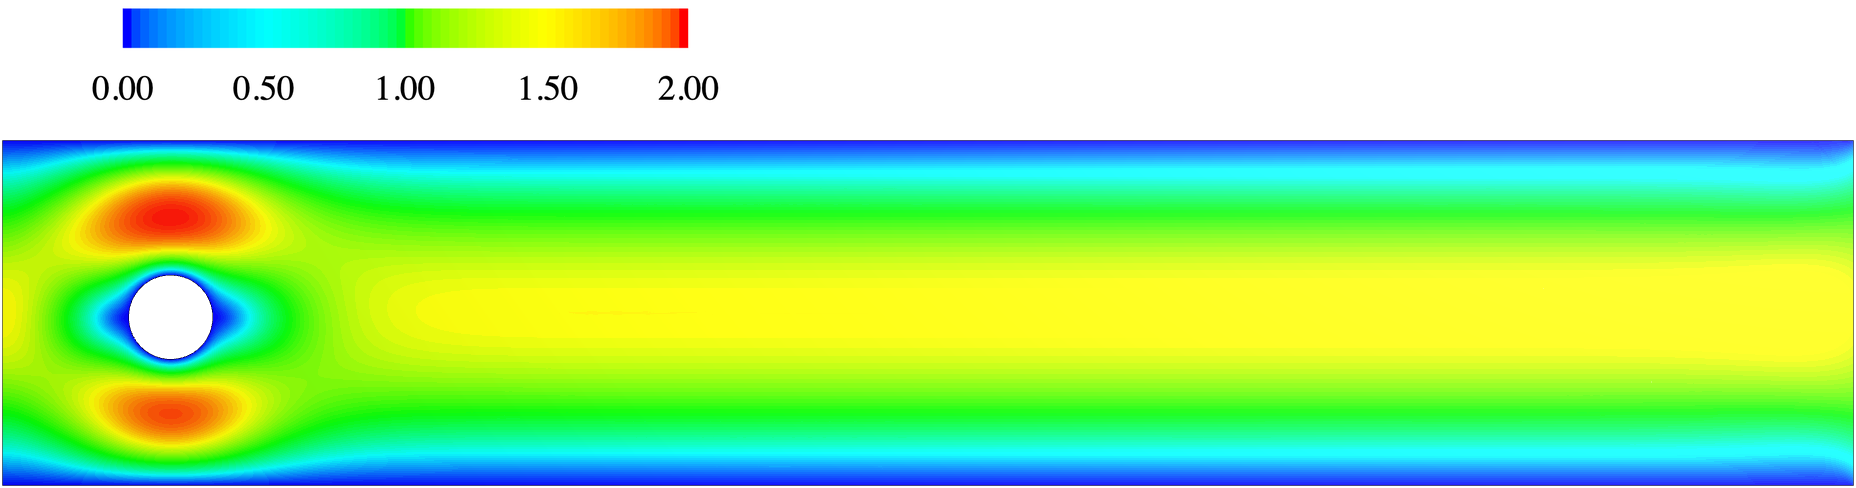
\includegraphics[width=\textwidth]{vel_c.png}\\[4pt]
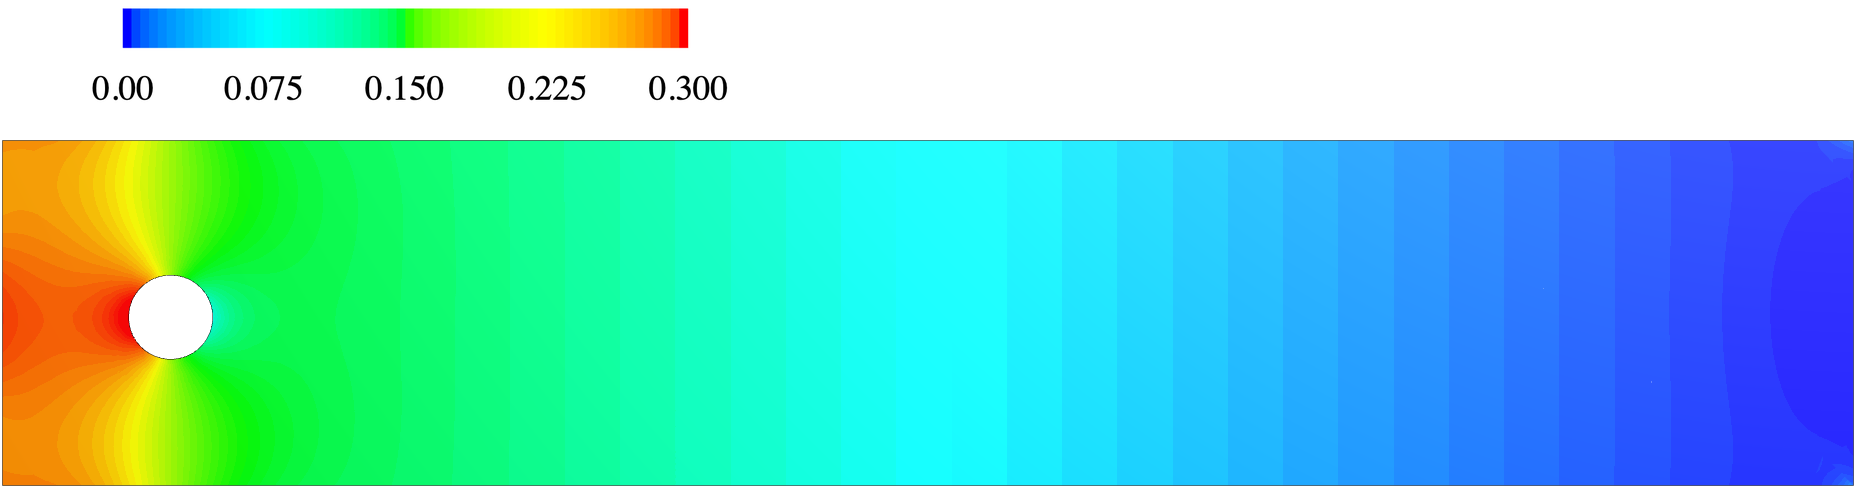
\includegraphics[width=\textwidth]{pres_c.png}
\end{minipage}\hfill
\begin{minipage}[c]{0.33\textwidth}\centering
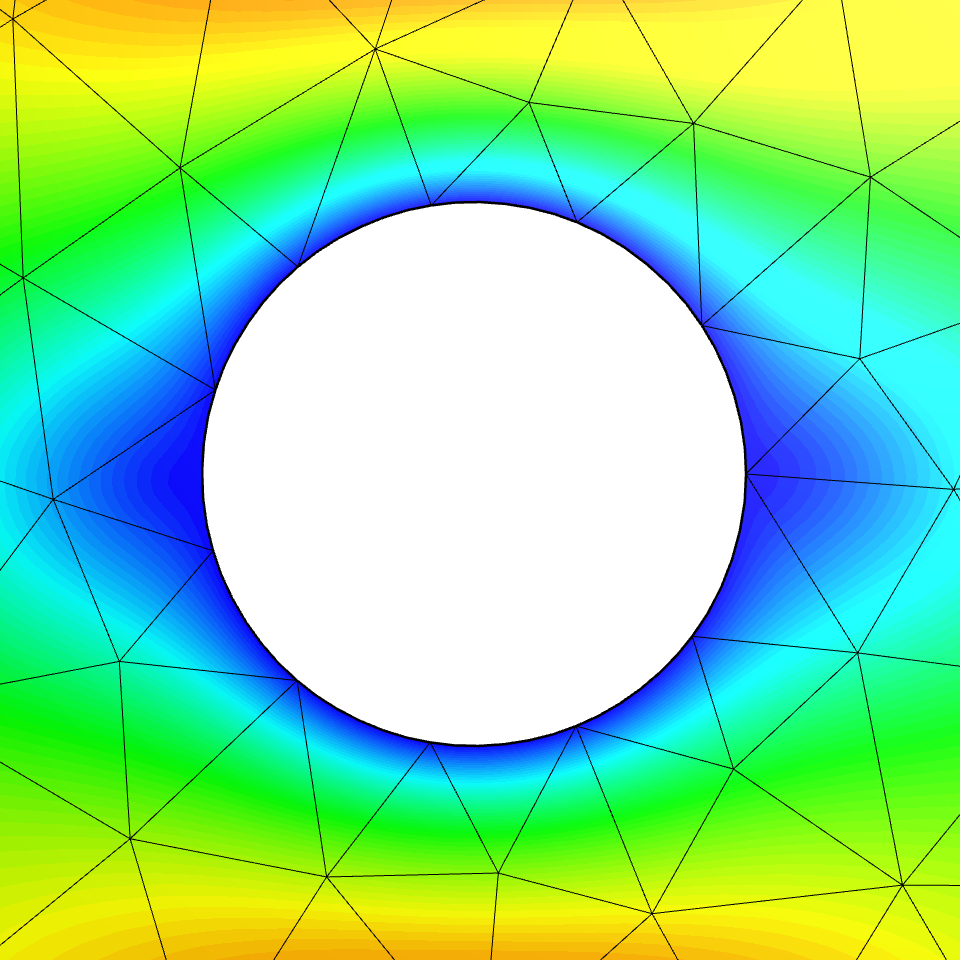
\includegraphics[width=\textwidth]{zoom_c.png}
\end{minipage}
\caption{Velocity magnitude $|u_h|$ (top left) and pressure $p_h$ (bottom left), drawn with \code{ngsolve.webgui} at visualization order 4 on the curved mesh (\code{mesh.Curve(3)}). Right: zoom on the cylinder with the curved elements. The pressure difference between the front and back of the cylinder is $p(0.15,0.2)-p(0.25,0.2) = 0.229$.}
\end{figure}

\section{Convergence and practical notes}

Manufactured solution $u = \operatorname{curl}\psi$ with $\psi = (x(1-x)y(1-y))^2$ on the unit square, and the analogous field on the unit cube. The pressure is $p = x - \tfrac12$. Weakly symmetric form, errors $\|u-u_h\|_{L^2}$ and $\|\dev(2\varepsilon(u)) - \sigma_h\|_{L^2}$, rates in brackets.

\begin{table}[h]\centering\footnotesize\setlength{\tabcolsep}{4pt}
\begin{tabular}{@{}llllll@{}}\toprule
 mesh & $k$ & $h=1/4$ & $1/8$ & $1/16$ & $1/32$\\\midrule
 trig (BDM) & 1 & 1.04e-3\ /\ 2.82e-2 & 2.49e-4 (2.1)\ /\ 1.47e-2 (0.9) & 5.31e-5 (2.2)\ /\ 7.07e-3 (1.1) & 1.35e-5 (2.0)\ /\ 3.55e-3 (1.0)\\
            & 2 & 2.34e-4\ /\ 7.92e-3 & 2.28e-5 (3.4)\ /\ 1.68e-3 (2.2) & 2.07e-6 (3.5)\ /\ 3.51e-4 (2.3) & 2.51e-7 (3.0)\ /\ 8.56e-5 (2.0)\\
            & 3 & 2.14e-5\ /\ 8.48e-4 & 1.14e-6 (4.2)\ /\ 9.28e-5 (3.2) & 6.00e-8 (4.2)\ /\ 1.12e-5 (3.1) & 3.20e-9 (4.2)\ /\ 1.18e-6 (3.2)\\\midrule
 mesh & $k$ & $h=1/2$ & $1/4$ & $1/8$ & \\\midrule
 prism (RT) & 1 & 1.72e-4\ /\ 3.06e-3 & 8.48e-5 (1.0)\ /\ 2.17e-3 (0.5) & 2.10e-5 (2.0)\ /\ 1.15e-3 (0.9) & \\
            & 2 & 9.26e-5\ /\ 1.87e-3 & 1.22e-5 (2.9)\ /\ 5.92e-4 (1.7) & 1.64e-6 (2.9)\ /\ 1.59e-4 (1.9) & \\\bottomrule
\end{tabular}
\caption{Velocity / stress errors. The velocity converges with order $k+1$ and the stress with order $k$. The coarse prism meshes ($h\ge 1/4$) are still pre-asymptotic.}
\end{table}

\paragraph{3D with boundary layers.}
The code is dimension independent. A duct with two prism boundary layers on the walls and tets inside needs a different geometry and \code{specialcf.normal(3)}; the rest stays the same:
\begin{lstlisting}
from netgen.occ import Box, X
from netgen.meshing import BoundaryLayerParameters

box = Box((0,0,0), (2,0.5,0.5))
box.faces.Min(X).name = "inlet"
box.faces.Max(X).name = "outlet"
box.faces[2:].name = "wall"
bl = BoundaryLayerParameters(boundary="wall", thickness=[0.02, 0.03])
mesh = box.GenerateMesh(maxh=0.15, boundary_layers=[bl])
# ... spaces and forms as above, n = specialcf.normal(3), k = 2
uin = CF((16*y*(0.5-y)*z*(0.5-z)/0.5**4, 0, 0))
gf = Solve(a == 0, u[BND("inlet|wall")] == uin, uhat[BND("inlet|wall")] == uin)
\end{lstlisting}
The mesh has 672 prisms and 506 tets, giving 239\,436 dofs; the solve takes 11\,s. The results are $\|\operatorname{div}u_h\|_{L^2} = 1\cdot10^{-14}$ and a net flux below $10^{-17}$ through the duct. The centreline velocity $0.93$ is that of the developed duct profile.

\paragraph{Practical notes.}
\begin{itemize}\setlength\itemsep{1pt}
\item \textbf{Boundary conditions.} \code{u[BND(..)] == g} sets the normal component, \code{uhat[BND(..)] == g} the tangential one. Both are needed for no-slip and inflow. Leaving a boundary out of both gives the do-nothing outflow.
\item \textbf{Pure Dirichlet problems.} The pressure is determined only up to a constant. Fix it, e.g.\ by a \code{NumberSpace} multiplier for $\int p = 0$ or a tiny $-\varepsilon\,(p,q)$ term.
\item \textbf{Exact mass conservation.} $\operatorname{div} u_h = 0$ holds pointwise because \code{Q} is exactly $\operatorname{div}$\code{V}. Mixing an RT velocity with a pressure of order $k-1$ loses this property; always use \code{CreateDivergenceSpace()}.
\item \textbf{Equivalence to the conforming method.} The hybrid and the conforming formulation (\code{S} instead of \code{Discontinuous(S)}, no \code{Vhat}) give the same $u_h$. On conforming stresses, $\hat u$ drops out of $b$.
\item \textbf{Interpolation.} \code{gf.Set(cf, dual=True)} uses the HCurlDiv dual basis (facet moments of $\tau_{nt}$ and interior moments). It reproduces discrete fields exactly, also on prisms and on curved or non-affine elements.
\item \textbf{Element support.} \code{CreateStressSpace} handles trigs, quads, tets, prisms and hexes, also on mixed meshes; pyramids raise an exception. The HCurlDiv prism is based on the element by X.~Mooslechner. Tet--prism interfaces are $\tau_{nt}$-conforming. Boundary values for $\hat u$ on quadrilateral faces (hexes, prism layers) are supported.
\end{itemize}

{\footnotesize\setlength{\itemsep}{0pt}
\begin{thebibliography}{9}\setlength{\itemsep}{1pt}
\bibitem{lederer} P.~L.~Lederer. \emph{A Mass Conserving Mixed Stress Formulation for Incompressible Flows}. PhD thesis, TU Wien, 2019.
\bibitem{gls1} J.~Gopalakrishnan, P.~L.~Lederer and J.~Sch\"oberl. A mass conserving mixed stress formulation for the Stokes equations. \emph{IMA J. Numer. Anal.} 40(3):1838--1874, 2020.
\bibitem{gls2} J.~Gopalakrishnan, P.~L.~Lederer and J.~Sch\"oberl. A mass conserving mixed stress formulation for Stokes flow with weakly imposed stress symmetry. \emph{SIAM J. Numer. Anal.} 58(1):706--732, 2020.
\bibitem{gg} J.~Gopalakrishnan and J.~Guzm\'an. A second elasticity element using the matrix bubble. \emph{IMA J. Numer. Anal.} 32(1):352--372, 2012.
\end{thebibliography}}

\end{document}
